\section{Procedure}
\begin{figure}[h]
    \centering
    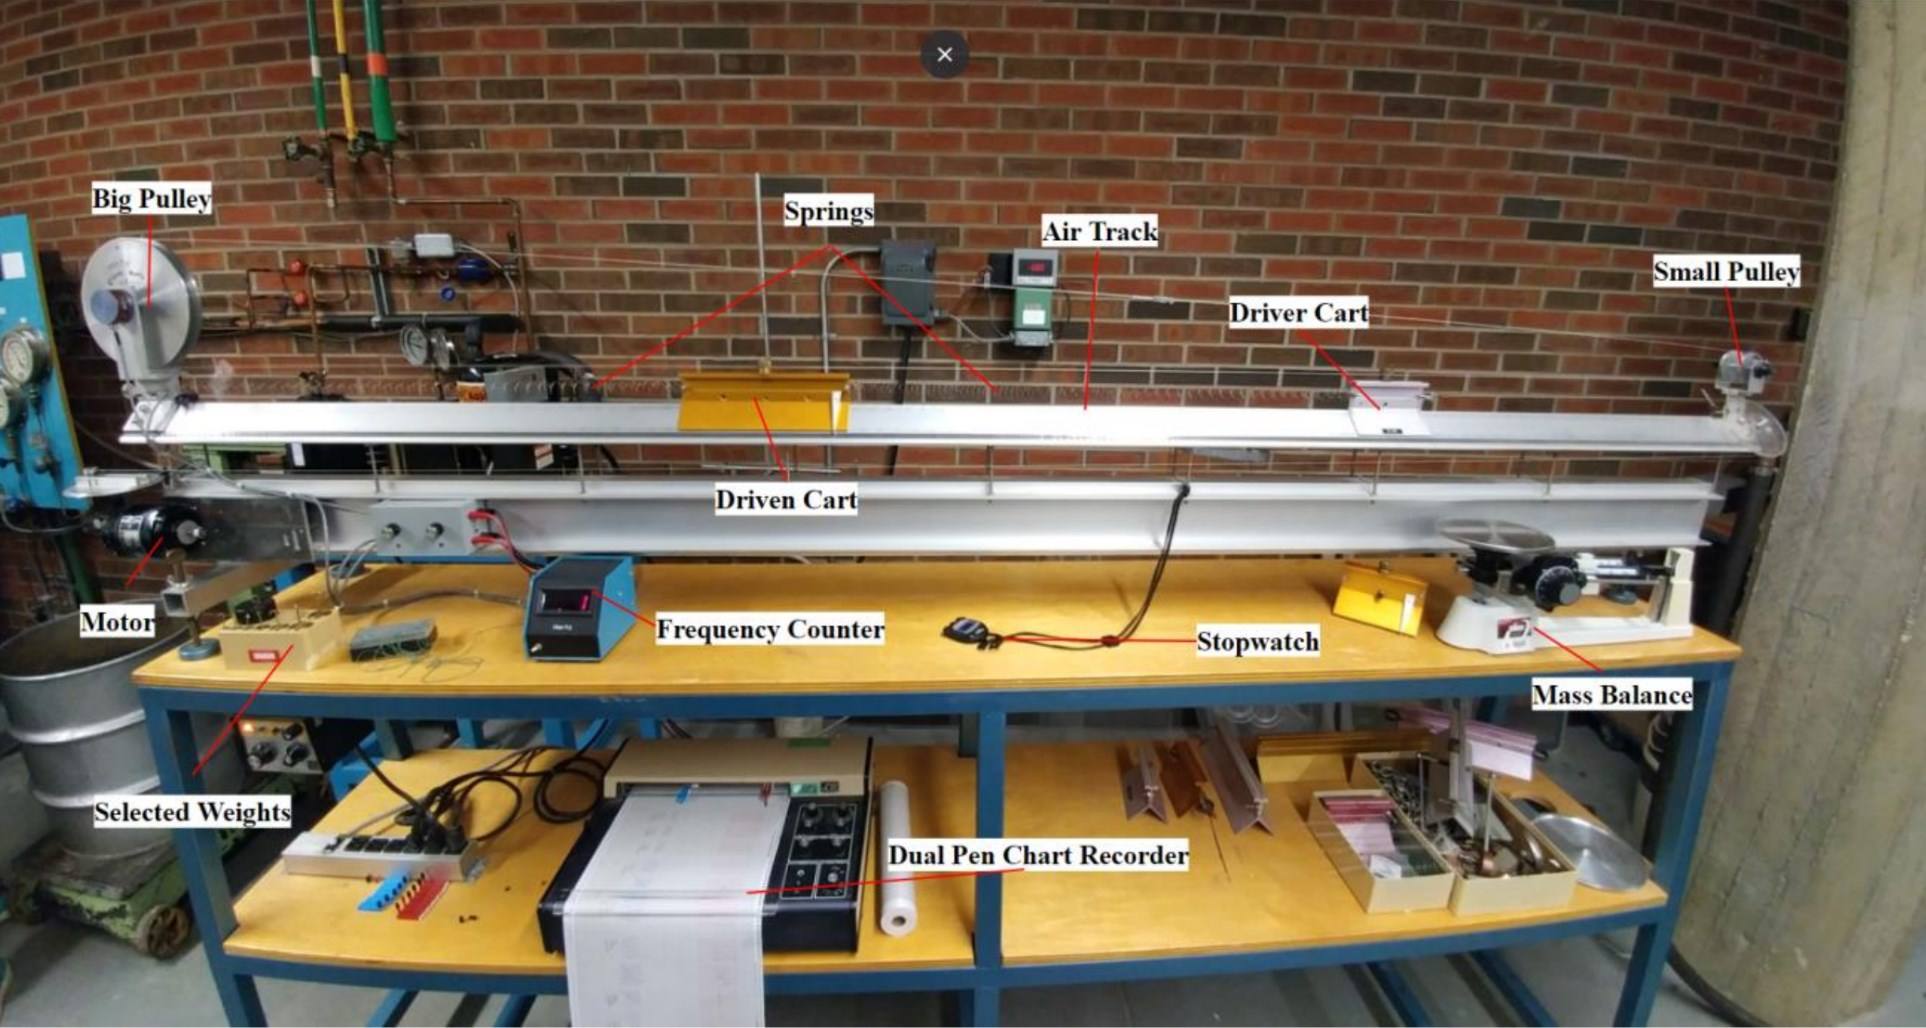
\includegraphics[width=0.5\textwidth]{Sections/Figures/experimental setup.jpg}
    \caption{Experimental Setup of the Spring-Mass System}
\end{figure}
\subsection{Equipment}
\begin{itemize}
    \item Air track, to provide a low friction surface for the carts
    \item Two springs, to provide an oscillatory response as the cart is displaced or driven
    \item Frequency counter, to measure the frequency of the forcing motor
    \item A large and small cart, to test the system with different masses
    \item Mass balance, to weigh the carts
    \item Motor and driver cart, to simulate a forced vibration system
    \item Pulleys, to record oscillations using software
    \item Stopwatch, to record the time of 10 oscillations
    \item Chart recorder, to record the oscillations of the system (not used in this experiment, software was used instead)
    \item Weights, to add to the cart to determine the load-deflection relationship of the system
    \item A pan, to hold the weights
\end{itemize}

% Shown above in Figure 1 is the lab apparatus used in this experiment. The air track provides a
% low friction surface (assumed frictionless) for the carts to glide along. The springs attached to the
% cart provide an oscillatory response as the cart is displaced or driven. The frequency counter
% measures this oscillatory response. Two carts of different mass (will be referred to as big and
% small) are tested, and weighed using the mass balance. The weights are added to the cart during
% testing to determine the load-deflection relationship of the system. The motor and driver cart are
% used to simulate a forced vibration system. The measurement system for this involves the
% pulleys, stopwatch, and chart recorder. The pulleys connect to the cart and record oscillations
% using software (note that this was used in place of the chart recorder). Finally, the stopwatch is
% used to record the time of 10 oscillations.

\subsection{Procedure}
\subsubsection{Load Deflection Trial}

\begin{enumerate}
    \item Record the mass of the cart by using the mass balance. Balance the beam by increasing and decreasing the weights on the other side of the beam until the beam is level. The mass of the cart will be used to determine the effective mass of the system for natural frequency calculations.
    \item Set the driving cart to a fixed position (i.e. undriven). This will reduce the system to a single degree of freedom.
    \item Detach the measurement system from the cart. This will allow the cart to oscillate freely.
    \item Turn on the air track to reduce friction between the cart and the track.
    \item Attach the cart to the pan around the free pulley. This will allow the cart to oscillate freely.
    \item Record the initial position of the cart. This will be used to determine the deflection of the cart.
    \item Add a 50 g weight to the pan. Record the new position of the cart. This will be used to determine the deflection of the cart.
    \item Repeat steps 7 and 8, increasing by 50 g until 300 g of weight is reached. This will be used to determine the load-deflection relationship and determine the effective stiffness of the system.
\end{enumerate}

\subsubsection{Free Vibrations}
\begin{enumerate}
    \item Remove the weights from the pan. This will allow the cart to oscillate freely.
    \item Give the cart an ~10cm initial deflection and then release it. This will allow the cart to oscillate freely.
    \item Record the time for the cart to complete ten oscillations using the stopwatch. This will be used to determine the natural frequency of the system.
    \item Repeat steps 2 and 3 five times to get an average value. This will be used to determine the natural frequency of the system.
    \item Redo steps 1-4 for the second, larger cart. This will be used to determine the natural frequency of the system for the larger cart.
\end{enumerate}

\subsubsection{Forced Vibrations}
\begin{enumerate}
    \item Attach the measurement system to the cart. This will allow the software to record the position of the cart.
    \item Attach the driving cart to the motor. This will allow the motor to drive the system.
    \item Turn on the motor and set the frequency below the determined natural frequency. This will allow the system to oscillate at a frequency below the natural frequency.
    \item Once steady state is reached, record the oscillations using the software for about 20 seconds. This will be used to determine the dynamic response of the system.
    \item Repeat steps 3 and 4 for four trials below the natural frequency and four trials above. This will be used to determine the dynamic response of the system.
    \item Redo steps 3-5 for the second, larger cart. This will be used to determine the dynamic response of the system for the larger cart.
\end{enumerate}